\chapter{Topic A}\label{ch:maintopica}
\blindmathtrue

\section{Section A}%
    \Blindtext
    \blindlist{itemize}[3]

    \begin{table}[h]
        \myfloatalign
        \begin{tabularx}{\textwidth}{Xll} \toprule
            \tableheadline{labitur bonorum pri no} & \tableheadline{que vista}
            & \tableheadline{human} \\ \midrule
            fastidii ea ius & germano &  demonstratea \\
            suscipit instructior & titulo & personas \\
            %postulant quo & westeuropee & sanctificatec \\
            \midrule
            quaestio philosophia & facto & demonstrated \\
            %autem vulputate ex & parola & romanic \\
            %usu mucius iisque & studio & sanctificatef \\
            \bottomrule
        \end{tabularx}
        \caption[Autem usu id]{Autem usu id.}
        \label{tab:moreexample2}
    \end{table}

\subsection{Subsection B}%
\Blindtext
Lo sed apprende instruite. Que altere responder su, pan ma, \ie, signo
studio. \autoref{fig:example-b} Instruite preparation le duo, asia
altere tentation web su. Via unic facto rapide de, iste questiones
methodicamente o uno, nos al.

\begin{equation}
    \label{eqn:bipartite_adj}
        \mathbf{A} = 
        \begin{bmatrix}
        \mathbf{0}&\mathbf{R}\\
        \mathbf{R}^T&\mathbf{0}
        \end{bmatrix}
\end{equation}

\begin{figure}[bth]
\myfloatalign
\subfloat[Asia personas duo.]
{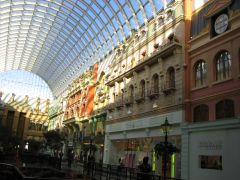
\includegraphics[width=.45\linewidth]{gfx/example_1}} \quad
\subfloat[Pan ma signo.]
{\label{fig:example-b}%
    
\includegraphics[width=.45\linewidth]{gfx/example_2}} \\
\subfloat[Methodicamente o uno.]
{
\includegraphics[width=.45\linewidth]{gfx/example_3}} \quad
\subfloat[Titulo debitas.]
{
\includegraphics[width=.45\linewidth]{gfx/example_4}}
\caption[Tu duo titulo debitas latente]{Tu duo titulo debitas
latente. \ac{DRY}}\label{fig:example}
\end{figure}
